\chapter{Existence of Nash Equilibrium}

\section{Non-existence of Nash Equilibrium}

The existence of a Nash equilibrium is not guaranteed. Several obstacles can prevent it.

\subsection{Examples of Non-existence}
\begin{enumerate}
    \item \textbf{Lack of compactness:} 2 players on $[0, +\infty[$, $u_1 = x_1$, $u_2 = x_2$. No equilibrium because payoffs are unbounded (everyone wants to play $+\infty$).
    \item \textbf{Lack of convexity or continuity (Continuous Matching Pennies):}
    This is the game "I like you, you don't like me". $u_1(x_1, x_2) = -|x_1 - x_2|$ (wants to get closer) and $u_2(x_1, x_2) = |x_1 - x_2|$ (wants to move away) on $[0,1]$.
    \begin{itemize}
        \item If $x_1 = x_2$, P2 wants to move away (play $0$ or $1$).
        \item If $x_1 \ne x_2$, P1 wants to get closer to $x_2$.
        \item There is no fixed point, so no pure strategy equilibrium.
    \end{itemize}
    
\begin{center}
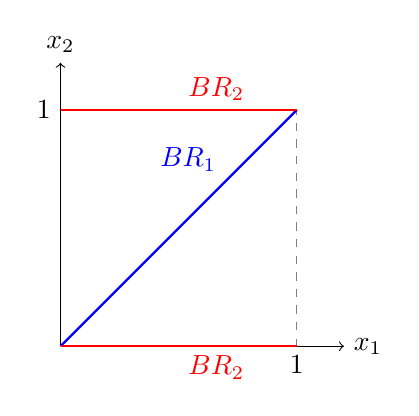
\begin{tikzpicture}[scale=3]
    % Axes
    \draw[->] (0,0) -- (1.2,0) node[right] {$x_1$};
    \draw[->] (0,0) -- (0,1.2) node[above] {$x_2$};
    % Unit square
    \draw[gray, dashed] (0,1) -- (1,1) -- (1,0);
    \node[below] at (1,0) {1};
    \node[left] at (0,1) {1};
    % BR1: x_1 = x_2 (diagonal)
    \draw[thick, blue] (0,0) -- (1,1);
    \node[blue, above left] at (0.7,0.7) {$BR_1$};
    % BR2: x_2 = 0 or x_2 = 1 (boundaries)
    \draw[thick, red] (0,0) -- (1,0);
    \draw[thick, red] (0,1) -- (1,1);
    \node[red, below right] at (0.5,0) {$BR_2$};
    \node[red, above right] at (0.5,1) {$BR_2$};
\end{tikzpicture}
\captionof{figure}{Continuous Matching Pennies: best responses never intersect.}
\end{center}
\begin{figureexplanation}
In this continuous zero-sum game on the square (Matching Pennies), the best responses (blue and red lines) never cross. There is therefore no intersection of the best response graphs, which implies that no pure strategy Nash equilibrium exists.
\end{figureexplanation}

\end{enumerate}

\begin{remarque}[Cultural Illustration]
The Professor often associates this frustration of non-existence with the painting \textbf{"The Scream" by Edvard Munch}: the anxiety of not finding a stable solution in a world without convexity or compactness.
\end{remarque}

\subsection{Obstacles to Existence}
The main obstacles to the existence of a Nash equilibrium are:
\begin{itemize}
    \item \textbf{Non-convex action sets:} In finite games, strategy sets have "holes".
    \item \textbf{Unbounded or non-closed action sets:} Compactness problem.
    \item \textbf{Discontinuous payoff functions.}
    \item \textbf{Lack of quasi-concavity:} If the payoff function is not quasi-concave, the set of best responses may not be convex.
\end{itemize}

\section{Quasiconcavity and Risk Appetite}

Quasi-concavity is a crucial property for existence. It is intimately linked to the notion of risk aversion or risk-seeking.

\begin{definition}[Quasiconcavity]
Let $X$ be a convex set. $f: X \rightarrow \mathbb{R}$ is \textbf{quasiconcave} if for all $\lambda \in [0,1]$ and all $(x, y) \in X^2$:
$$f(\lambda x + (1-\lambda)y) \ge \min\{f(x), f(y)\}$$
\textbf{Equivalent characterization:} $f$ is quasiconcave if and only if all its \textbf{upper level sets} are convex:
$$\forall \alpha \in \mathbb{R}, \quad S_{\alpha}(f) = \{x \in X : f(x) \ge \alpha\} \text{ is convex.}$$
\end{definition}

\begin{exemple}[Economic Intuition: Risk-Loving]
Consider $u(x) = x^2$ on $\mathbb{R}$.
\begin{itemize}
    \item This function is convex (parabola).
    \item It is \textbf{not quasiconcave} on $\mathbb{R}$ (e.g., $S_1(f) = ]-\infty, -1] \cup [1, +\infty[$ is not convex).
    \item \textbf{Interpretation:} An agent with such utility is "Risk-Loving". They prefer an uncertain outcome (e.g., a lottery between -2 and 2, mean 0) to its certain equivalent (0), because $u(0)=0 < 0.5 u(-2) + 0.5 u(2) = 4$.
\end{itemize}

\begin{center}
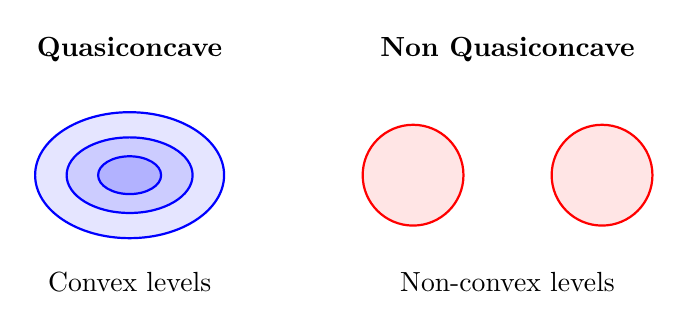
\begin{tikzpicture}[scale=0.8]
    % Quasiconcave (left)
    \node at (2, 3.5) {\textbf{Quasiconcave}};
    \draw[thick, blue, fill=blue!10] (2,1.5) ellipse (1.5 and 1);
    \draw[thick, blue, fill=blue!20] (2,1.5) ellipse (1 and 0.6);
    \draw[thick, blue, fill=blue!30] (2,1.5) ellipse (0.5 and 0.3);
    \node at (2, -0.2) {Convex levels};
    
    % Not quasiconcave (right)
    \node at (8, 3.5) {\textbf{Non Quasiconcave}};
    \draw[thick, red, fill=red!10] (6.5,1.5) ellipse (0.8 and 0.8);
    \draw[thick, red, fill=red!10] (9.5,1.5) ellipse (0.8 and 0.8);
    \node at (8, -0.2) {Non-convex levels};
\end{tikzpicture}
\captionof{figure}{Upper level sets: convex (quasiconcave) vs non-convex.}
\end{center}
\begin{figureexplanation}
Quasi-concavity is characterized by the convexity of upper level sets $S_\alpha = \{x \mid f(x) \ge \alpha\}$.
\begin{itemize}
    \item Left: $S_\alpha$ (colored zones) is always convex. The function is quasi-concave.
    \item Right: For some $\alpha$, $S_\alpha$ is disjoint (union of two separate sets), so not convex. The function is not quasi-concave.
\end{itemize}
\end{figureexplanation}

\end{exemple}

\section{Glicksberg's Theorem}
This is the fundamental theorem ensuring the existence of a Nash equilibrium in pure strategies.

\begin{theoreme}[Glicksberg]
Let a game $G = (N, (X_i)_{i \in N}, (u_i)_{i \in N})$ such that:
\begin{enumerate}
    \item $X_i$ is a \textbf{compact and convex} subset of a topological vector space.
    \item $u_i$ is \textbf{continuous} on $X = \prod X_i$.
    \item $x_i \mapsto u_i(x_i, x_{-i})$ is \textbf{quasiconcave} for all $x_{-i}$.
\end{enumerate}
Then, there exists a Nash equilibrium.
\end{theoreme}

\subsection{Proof (Exam Rigor)}
The proof relies on applying the fixed point theorem to the best response correspondence $B(x) = \prod B_i(x_{-i})$.

\paragraph{Why Kakutani and not Brouwer?}
Brouwer's Theorem applies to continuous \textbf{functions}. Here, the best response is not unique (it's a set), it is a \textbf{correspondence}. We must therefore use \textbf{Kakutani's Theorem}.

\begin{center}
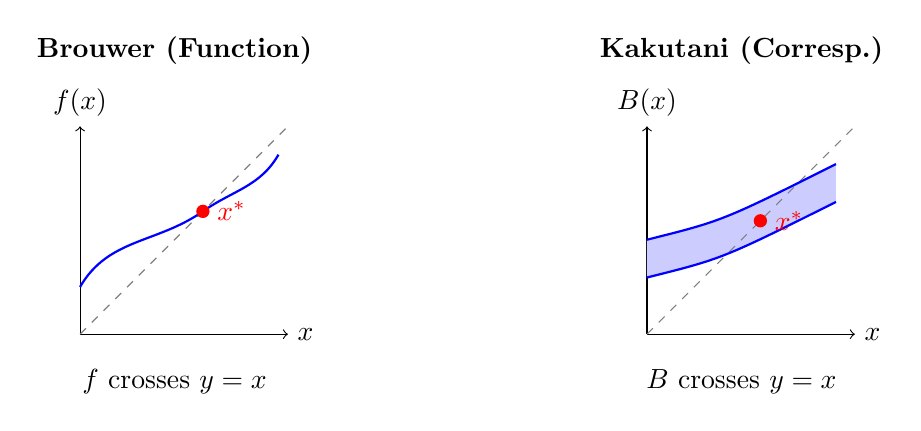
\begin{tikzpicture}[scale=1.2]
    % Brouwer (left)
    \begin{scope}[shift={(-3.5,0)}]
        \node at (1, 3.0) {\textbf{Brouwer (Function)}};
        \draw[->] (0,0) -- (2.2,0) node[right] {$x$};
        \draw[->] (0,0) -- (0,2.2) node[above] {$f(x)$};
        \draw[gray, dashed] (0,0) -- (2.2,2.2);
        
        % Curve adjusted to cross exactly at (1.3, 1.3)
        \draw[thick, blue] (0,0.5) to[out=60, in=215] (1.3,1.3) to[out=35, in=240] (2.1,1.9);
        
        \fill[red] (1.3,1.3) circle (2pt);
        \node[red, right] at (1.35,1.3) {$x^*$};
        \node at (1,-0.5) {$f$ crosses $y=x$};
    \end{scope}
    
    % Kakutani (right)
    \begin{scope}[shift={(2.5,0)}]
        \node at (1, 3.0) {\textbf{Kakutani (Corresp.)}};
        \draw[->] (0,0) -- (2.2,0) node[right] {$x$};
        \draw[->] (0,0) -- (0,2.2) node[above] {$B(x)$};
        
        % Correspondence as a convex-valued band
        \fill[blue!20] (0,0.6) .. controls (0.8,0.8) .. (2,1.4) 
            -- (2,1.8) .. controls (0.8,1.2) .. (0,1.0) -- cycle;
            
        % Dashed line (diagonal) - DRAWN AFTER FILL for visibility
        \draw[gray, dashed] (0,0) -- (2.2,2.2);

        % Border lines of the correspondence
        \draw[thick, blue] (0,0.6) .. controls (0.8,0.8) .. (2,1.4);
        \draw[thick, blue] (0,1.0) .. controls (0.8,1.2) .. (2,1.8);
        
        % Fixed point intersection
        \fill[red] (1.2,1.2) circle (2pt);
        \node[red, right] at (1.25,1.2) {$x^*$};
        
        \node at (1,-0.5) {$B$ crosses $y=x$};
    \end{scope}
\end{tikzpicture}
\captionof{figure}{Brouwer vs Kakutani: function vs correspondence.}
\end{center}
\begin{figureexplanation}
\textbf{Comparison of theorems:}
\begin{itemize}
    \item \textbf{Brouwer (Left):} If $f$ is a continuous \textit{function} from $[0,1]$ to itself, its graph (blue curve) must necessarily cross the diagonal (dashed). The intersection is a fixed point $x^* = f(x^*)$.
    \item \textbf{Kakutani (Right):} If $B$ is a \textit{correspondence} (set of values) with closed graph and convex values (the blue zone is "solid" vertically), its graph must also cross the diagonal. The intersection $x^*$ satisfies $x^* \in B(x^*)$, it is a fixed point.
\end{itemize}
\end{figureexplanation}

\paragraph{Verification of Kakutani's 3 conditions:}
To apply Kakutani to $B : X \rightrightarrows X$, we must verify:
\begin{enumerate}
    \item \textbf{Non-empty:} Since $u_i$ is continuous on a compact set $X_i$, it reaches its maximum (Weierstrass Theorem). So $B_i(x_{-i}) \ne \emptyset$.
    \item \textbf{Convex values:} Since $u_i$ is quasi-concave with respect to $x_i$, the set of maximizers $B_i(x_{-i})$ is convex.
    \item \textbf{Closed Graph:} This is a consequence of the global continuity of $u_i$ (Berge's Maximum Theorem). If a sequence $x^n \to x$ and $y^n \in B(x^n)$ with $y^n \to y$, then $y \in B(x)$.
\end{enumerate}
All conditions being met, $B$ admits a fixed point $x^* \in B(x^*)$, which is a Nash equilibrium.

\section{Solved Examples}

\subsection{Public Good Provision}
For $n$ inhabitants, $u_i = W - x_i + \sqrt{\sum x_j}$. We look for a symmetric equilibrium $(a, \dots, a)$.
Let $f(x_i) = W - x_i + \sqrt{(n-1)a + x_i}$. The first order condition $f'(a) = 0$ gives:
$$-1 + \frac{1}{2\sqrt{na}} = 0 \iff 2\sqrt{na} = 1 \iff 4na = 1 \iff a = \frac{1}{4n}$$

\subsection{Rent-seeking (Tullock)}
$n$ firms, payoff $u_i = \frac{x_i}{\sum x_j}V - cx_i$. For a symmetric equilibrium $a$:
$$f'(x_i) = \frac{V((n-1)a + x_i) - Vx_i}{((n-1)a + x_i)^2} - c = 0$$
At $x_i = a$, we get $\frac{(n-1)V}{n^2 a} = c$, so $a = \frac{n-1}{cn^2}V$.

\section{Extensions and Limiting Cases (Further Reading)}

\begin{itemize}
    \item \textbf{Coercivity Argument:} If action sets are not compact (e.g., $X_i = \mathbb{R}$), an equilibrium can still exist if functions are \textbf{coercive}, i.e., if $\lim_{|x_i| \to \infty} u_i(x) = -\infty$. This allows restricting analysis to a sufficiently large compact subset.
\end{itemize}

\begin{exemple}[Exam 2023: Proof of Coercivity]
\textbf{Question:}
Prove the existence of a Nash equilibrium for a game where utility functions are coercive.

\textbf{Solution:}
\begin{enumerate}
    \item By hypothesis, $\lim_{|x| \to \infty} u_i(x, y) = -\infty$. The function is therefore coercive on a closed set, which guarantees the existence of a maximum and thus a best response.
    \item By considering a sequence of games on compact sets $X_n \times Y_n$, we apply Glicksberg's theorem to guarantee the existence of a Nash equilibrium $(\bar{x}_n, \bar{y}_n)$.
    \item Since the best responses are bounded by coercivity, the sequence converges to an equilibrium $(\bar{x}, \bar{y})$ of the original game.
\end{enumerate}
\end{exemple}

\subsection{Remarks on Existence (Beyond Exam Scope)}
In many economic models, payoff functions are discontinuous. The existence of a Nash equilibrium can still be guaranteed under certain conditions:
\begin{itemize}
    \item \textbf{Reny (1999)}: Concept of "better-reply security".
    \item \textbf{Bich-Laraki (2017)}: Work on games with discontinuous payoffs.
    \item \textbf{Bich (2004)}: Non-continuous version of Brouwer's fixed point theorem.
\end{itemize}

\paragraph{Consensus Game}
Three players $i \in \{1,2,3\}$, $X_i = [0,1]$.
\[ u_1(x_1, x_2, x_3) = - \left| x_1 - \frac{x_2 + x_3}{2} \right|^2 \]
Each player seeks to be as close as possible to the average of the others.
The equilibrium is $(1/2, 1/2, 1/2)$ if looking for a fixed point.

\begin{exercice}[Symmetric Nash Equilibrium]
Let $G = (X, X, u, u)$ be a symmetric game where $X$ is compact convex and $u$ is continuous and quasi-concave with respect to its first variable. Prove using Kakutani's theorem applied to the best response correspondence $BR$ that there exists a symmetric equilibrium $(x^*, x^*)$.
\paragraph{Solution:}
1. Let $BR : X \rightrightarrows X$ be the best response correspondence of the representative player.
2. Define the function $\phi : X \to \mathcal{P}(X)$ by $\phi(x) = BR(x, x, \dots, x)$.
   
   \textbf{Simpler method:}
   Let the "symmetric best-reply reaction" correspondence $F: X \rightrightarrows X$ be defined by:
   $$ y \in F(x) \iff y \in \arg\max_{z \in X} u(z, x, \dots, x) $$
   ($y$ is the best response of a player if ALL others play $x$).
   
   \begin{itemize}
       \item $X$ is non-empty compact convex.
       \item $F(x)$ is non-empty (continuity on compact) and convex (quasi-concavity).
       \item $F$ has a closed graph (Maximum Theorem).
   \end{itemize}
   By Kakutani's Theorem, $F$ admits a fixed point $x^* \in F(x^*)$.
   This means that if all others play $x^*$, the best response for me is also to play $x^*$.
   Since the game is symmetric, $(x^*, \dots, x^*)$ is a Nash equilibrium.
\end{exercice}

\section{Conclusion and Transition}
We have seen that the existence of a Nash equilibrium in pure strategies requires strong conditions (convexity, continuity, quasi-concavity). When these conditions are not met (for example, in finite games where discrete action sets are not convex), a pure strategy equilibrium may not exist (e.g., Matching Pennies, Rock-Paper-Scissors).

To guarantee the existence of a stable solution in all finite games, we must extend our concept of strategy and allow players to randomize their choices. This is the subject of the next chapter on \textbf{mixed strategies}.
